\subsection{SubBytes transformation}
\label{sec:sub-bytes}

SubBytes transformation can be implemented in two ways
\begin{itemize}[nolistsep]
\item As a look-up table of precomputed values stored in on-chip memory
\item As combinatorial logic circuit.
\end{itemize}
This section will discuss advantages, disadantages and implementation details of both approaches.

\subsubsection{Look-up table approach}
SubBytes transformation can be implemented as a look-up table of precomputed values (\cite[Fig. 7]{aes-standard}). Implementing it this way is simple and resource efficient, but has a major limitation -- it can operate only as fast as on-chip memory, which in case of DE1-SoC FPGA device is 300MHz. This limits the overall throughput of AES encryption to
$$
300MHz * 16B = 4.8GB/s
$$
This approach can be considered for resource-optimized hardware implementations of AES algorithm, but its maximum achievable throughput is not high enough for performace-optimized versions.


\subsubsection{Combinatorial logic approach}
\label{sec:comb-theory}
Alternative approach to implementing SubBytes transformation is to not store any precomputed byte substitutions in on-chip memory and use combinatorial logic to calculate them instead. This method is not limited by frequency of memory and therefore capable of achieving better throughut. It is however significantly more complex and uses more FPGA logic elements. It is therefore suitable for performance optimized AES architectures, but not for resource-optimized ones.

\paragraph{Top level design of SubBytes transformation}\mbox{}\\
As defined in AES standard \cite{aes-snadard} SubBytes transformation consists of
\begin{itemize}[nolistsep]
\item Multiplicative inversion in $GF(2^8)$
\item Affine transformation specified in AES standard \cite{aes-standard}
\end{itemize}
Calculating multiplicative inversion is the most demanding part of this transformationa and naively implementing it in $GF(2^8)$ would require at least 620 gates (\cite{vlsi}). This number can be gratly reduced by using composite field arithmetic. To achieve this SubBytes transformation can be decomposed into stages (details explained in following paragraphs):
\begin{enumerate}[nolistsep]
\item Map input byte from $GF(2^8)$ to $GF((2^4)^2)$ 
\item calculate multiplicative inverse in $GF((2^4)^2)$
\item Map byte from $GF((2^4)^2)$ back to $GF(2^8)$
\item Apply affine transformation defined in AES standard \cite{aes-standard}
\end{enumerate}



\begin{figure}[!h]
\label{fig:sub-single-byte}
\centering
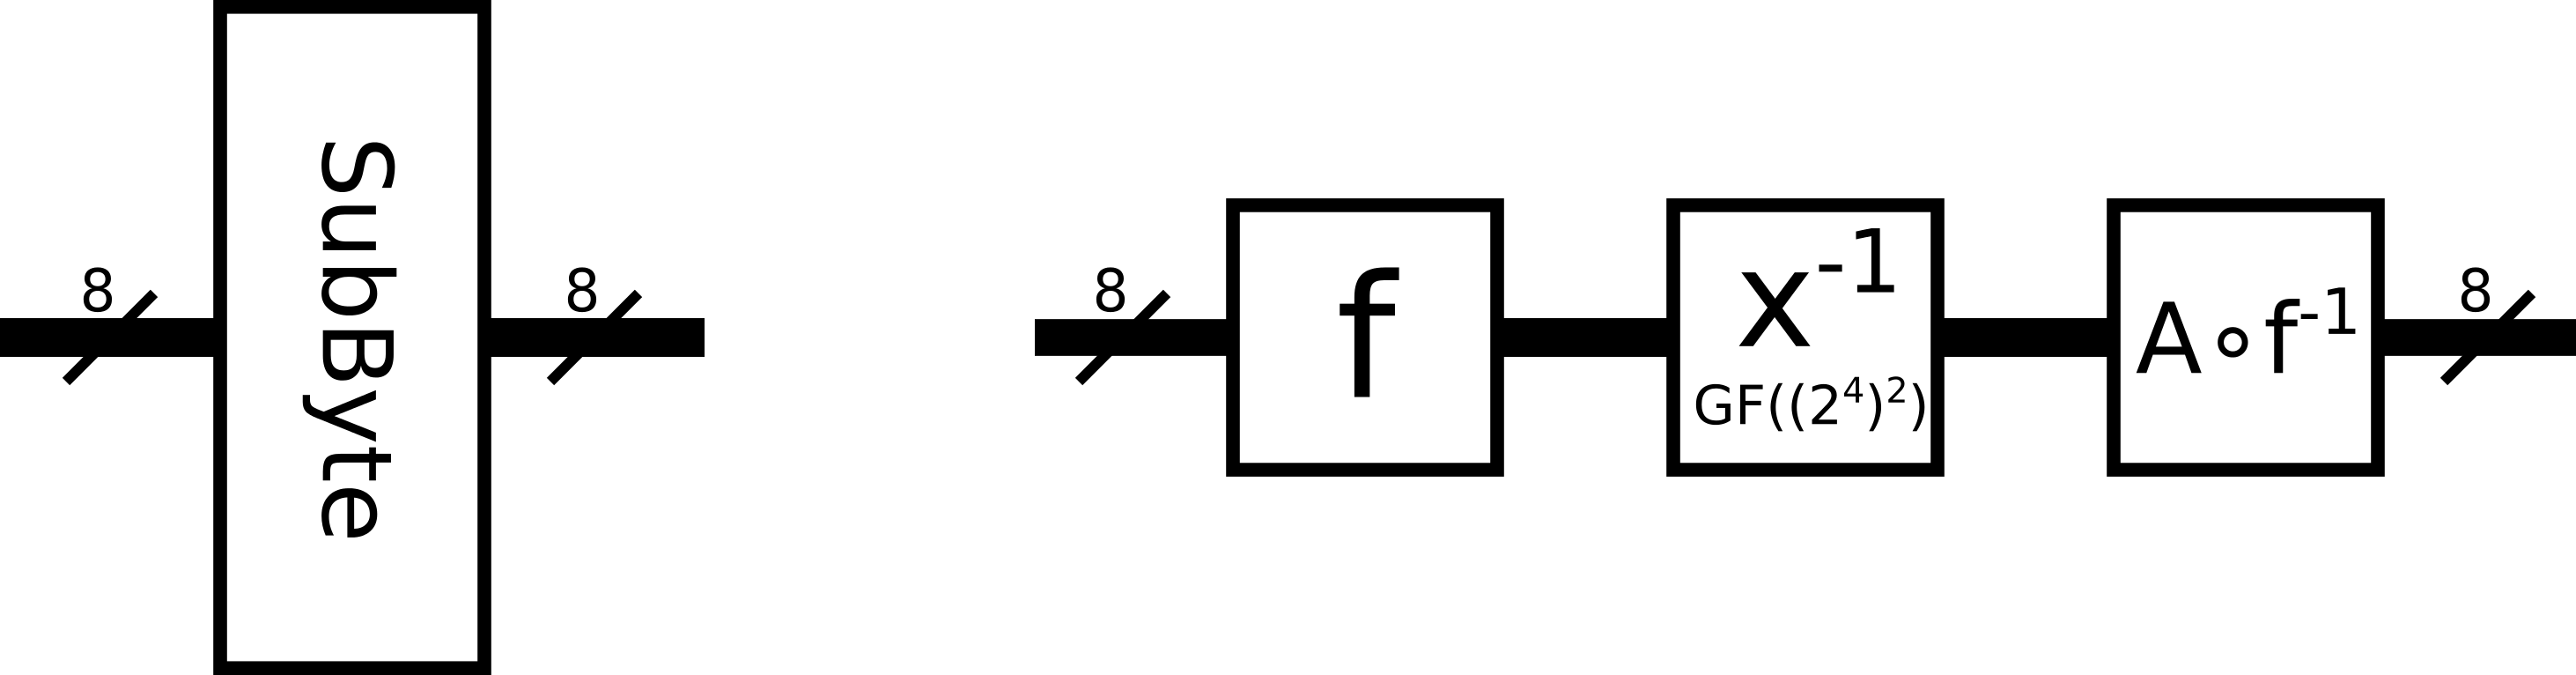
\includegraphics[scale=3]{sub-bytes}
\caption{SubButes transformation}
\end{figure}

Steps 3 and 4 can be joined into a single operation. SubBytes transformation for single byte can be implemented as a circuit in figure \ref{fig:sub-single-byte}. SubBytes transformation for entire state requires 16 such blocks. Detailed information about all required operations can be found in following paragraphs.

\paragraph{Composite Galois Fields and mapping between $GF(2^8)$ and $GF((2^4)^2)$}\mbox{}\\
We call two pairs
\begin{equation*}
\{GF(2^n), Q(y) = y^n + \sum_{i=0}^{n-1} q_i y^i, q_i \in GF(2) \}
\end{equation*}
\begin{equation*}
\{GF((2^n)^m), P(x) = x^m + \sum_{i=0}^{m-1} p_i x^i, p_i \in GF(2^n) \}
\end{equation*}
a composite field \cite{vlsi} if 
\begin{itemize}[nolistsep]
\item $GF(2^n)$ is constructed from $GF(2)$ by $Q(y)$
\item $GF((2^n)^m)$ is constructed from $GF(2^n)$ by $P(x)$
\end{itemize}
A composite field $GF((2^n)^m)$ is isomorphic to the field $GF(2^k)$ for $k = nm$ \cite{vlsi}.

For SubBytes transformation we will use the following composite fields and polynomials \cite{vlsi}:

\begin{equation}
\begin{aligned}
\label{eq:comp_fields_and_polys}
&GF(2) \Rightarrow GF(2^2) :               & P_0(x) = x^2 + x + 1\\
&GF(2^2) \Rightarrow GF((2^2)^2) :         & P_1(x) = x^2 + x + \phi\\
&GF((2^2)^2) \Rightarrow GF(((2^2)^2)^2) : & P_2(x) = x^2 + x + \lambda
\end{aligned}
\end{equation}

where $\phi = \{10\}$ and $\lambda = \{1100\}$.

An isomorphic mapping function $f(x)$ (\ref{eq:iso_map}) from $GF(2^8)$ to $GF((2^4)^2)$ can be found by exhaustive-search-based algorithm \cite{vlsi}. $\delta$ matrix corresponds to $p(x) = x^8 + x^4 + x^3 + x + 1$ (irreducible polynomial for $GF(2^8)$ defined in AES standard \cite{aes-standard}) and the polynomials in (\ref{eq:comp_fields_and_polys}). Reverse mapping from $GF((2^4)^2)$ to $GF(2^8)$ can be done with $f^{-1}(x)$ function (\ref{eq:iso_map_rev}).

\begin{equation}
\begin{gathered}
\label{eq:iso_map}
f(x) = \delta * x\\
x \in GF(2^8), f(x) \in GF((2^4)^2) \\
\begin{bmatrix}
b_0'\\b_1'\\b_2'\\b_3'\\b_4'\\b_5'\\b_6'\\b_7'
\end{bmatrix}
=
\begin{bmatrix}
    1 & 1 & 0 & 0 & 0 & 0 & 1 & 0 \\
    0 & 1 & 0 & 0 & 1 & 0 & 1 & 0 \\
    0 & 1 & 1 & 1 & 1 & 0 & 0 & 1 \\
    0 & 1 & 1 & 0 & 0 & 0 & 1 & 1 \\
    0 & 1 & 1 & 1 & 0 & 1 & 0 & 1 \\
    0 & 0 & 1 & 1 & 0 & 1 & 0 & 1 \\
    0 & 1 & 1 & 1 & 1 & 0 & 1 & 1 \\
    0 & 0 & 0 & 0 & 0 & 1 & 0 & 1
\end{bmatrix}
\begin{bmatrix}
b_0\\b_1\\b_2\\b_3\\b_4\\b_5\\b_6\\b_7
\end{bmatrix}
\end{gathered}
\end{equation}

\begin{equation}
\begin{gathered}
\label{eq:iso_map_rev}
f^{-1}(x) = \delta^{-1} * x\\
x \in GF((2^4)^2), f^{-1}(x) \in GF(2^8) \\
\begin{bmatrix}
b_0'\\b_1'\\b_2'\\b_3'\\b_4'\\b_5'\\b_6'\\b_7'
\end{bmatrix}
=
\begin{bmatrix}
    1 & 0 & 1 & 0 & 1 & 1 & 1 & 0 \\
    0 & 0 & 0 & 0 & 1 & 1 & 0 & 0 \\
    0 & 1 & 1 & 1 & 1 & 0 & 0 & 1 \\
    0 & 1 & 1 & 1 & 1 & 1 & 0 & 0 \\
    0 & 1 & 1 & 0 & 1 & 1 & 1 & 0 \\
    0 & 1 & 0 & 0 & 0 & 1 & 1 & 0 \\
    0 & 0 & 1 & 0 & 0 & 0 & 1 & 0 \\
    0 & 1 & 0 & 0 & 0 & 1 & 1 & 1
\end{bmatrix}
\begin{bmatrix}
b_0\\b_1\\b_2\\b_3\\b_4\\b_5\\b_6\\b_7
\end{bmatrix}
\end{gathered}
\end{equation}

A value $v = \{b_{2^n-1}...b_0\} \in GF((2^n)^2)$ is interpreted as a polynomial $p(x) = \sum_{i=0}^{n-1} b_ix^i$, where $b_i \in GF(2) = \{0, 1\}$ are bits. Any value $v \in GF((2^n)^2)$ can be represented as \cite{vlsi}:
\begin{equation}
\label{eq:poly_repr}
v = v_hx + v_l
\end{equation}
where $v_h = \{b_{2^n-1}...b_{2^{n-1}}\} \in GF(2^n)$ (high bits) and $v_l = \{b_{2^{n-1}-1}...b_0\} \in GF(2^n)$ (low bits). This holds true for decomposing values in $GF((2^n)^2)$ for any $n > 0$.

\paragraph{Affine transformation}\mbox{}\\
In SubBytes transformation, last step of calculating multiplicative inversion in $GF(2^8)$ is mapping $f^{-1}(x)$ from $GF((2^4)^2)$ to $GF(2^8)$. Immediately after this operation an affine transformation $a(x)$ is applied.
\begin{equation}
\begin{gathered}
\label{eq:affine}
a(x) = A * x + B\\
x \in GF(2^8), a(x) \in GF(2^8) \\
\begin{bmatrix}
b_0'\\b_1'\\b_2'\\b_3'\\b_4'\\b_5'\\b_6'\\b_7'
\end{bmatrix}
=
\begin{bmatrix}
    1 & 0 & 0 & 0 & 1 & 1 & 1 & 1 \\
    1 & 1 & 0 & 0 & 0 & 1 & 1 & 1 \\
    1 & 1 & 1 & 0 & 0 & 0 & 1 & 1 \\
    1 & 1 & 1 & 1 & 0 & 0 & 0 & 1 \\
    1 & 1 & 1 & 1 & 1 & 0 & 0 & 0 \\
    0 & 1 & 1 & 1 & 1 & 1 & 0 & 0 \\
    0 & 0 & 1 & 1 & 1 & 1 & 1 & 0 \\
    0 & 0 & 0 & 1 & 1 & 1 & 1 & 1
\end{bmatrix}
\begin{bmatrix}
b_0\\b_1\\b_2\\b_3\\b_4\\b_5\\b_6\\b_7
\end{bmatrix}
+
\begin{bmatrix}
1\\1\\0\\0\\0\\1\\1\\0
\end{bmatrix}
\end{gathered}
\end{equation}

As mapping $f^{-1}(x)$ from $GF((2^4)^2)$ to $GF(2^8)$ and affine transformation $a(x)$ are matrix multiplications, those two operations can be combined.
\begin{equation}
\begin{gathered}
\label{eq:affine}
f \circ a(x) = A * \delta * x + B\\
x \in GF(2^8), f \circ a(x) \in GF(2^8) \\
\begin{bmatrix}
b_0'\\b_1'\\b_2'\\b_3'\\b_4'\\b_5'\\b_6'\\b_7'
\end{bmatrix}
=
\begin{bmatrix}
    1 & 1 & 1 & 0 & 0 & 0 & 1 & 1 \\
    1 & 0 & 0 & 0 & 0 & 0 & 0 & 1 \\
    1 & 0 & 1 & 1 & 1 & 1 & 1 & 0 \\
    1 & 1 & 1 & 0 & 0 & 0 & 0 & 0 \\
    1 & 1 & 0 & 0 & 1 & 0 & 0 & 1 \\
    0 & 0 & 1 & 0 & 0 & 0 & 0 & 1 \\
    0 & 0 & 0 & 0 & 1 & 1 & 1 & 1 \\
    0 & 0 & 1 & 1 & 0 & 0 & 0 & 1
\end{bmatrix}
\begin{bmatrix}
b_0\\b_1\\b_2\\b_3\\b_4\\b_5\\b_6\\b_7
\end{bmatrix}
+
\begin{bmatrix}
1\\1\\0\\0\\0\\1\\1\\0
\end{bmatrix}
\end{gathered}
\end{equation}



\paragraph{Multiplicative inversion in $GF((2^4)^2)$}\mbox{}\\
In \cite{vlsi}[APPENDIX] it is proven that multiplicative inversion of $v = v_hx + v_l \in GF((2^4)^2)$ modulo $P_2(x)$ (\ref{eq:comp_fields_and_polys}) can be computed as in (\ref{eq:inv_formula_gf242}):
\begin{equation}
\begin{gathered}
\label{eq:inv_formula_gf242}
(v_hx + v_l)^{-1} = s_h \Theta x + (s_h + s_l) \Theta\\
\Theta = (s_h^2 \lambda + s_hs_l + s_l^2)^{-1} = (s_h^2 \lambda + s_l (s_h + s_l))^{-1}
\end{gathered}
\end{equation}

$\Theta$ and entire inversion can be implemented as circuits in figures \ref{fig:theta_impl} and \ref{fig:mul_inv_gf242}.

\begin{figure}
\label{fig:theta_impl}
\centering
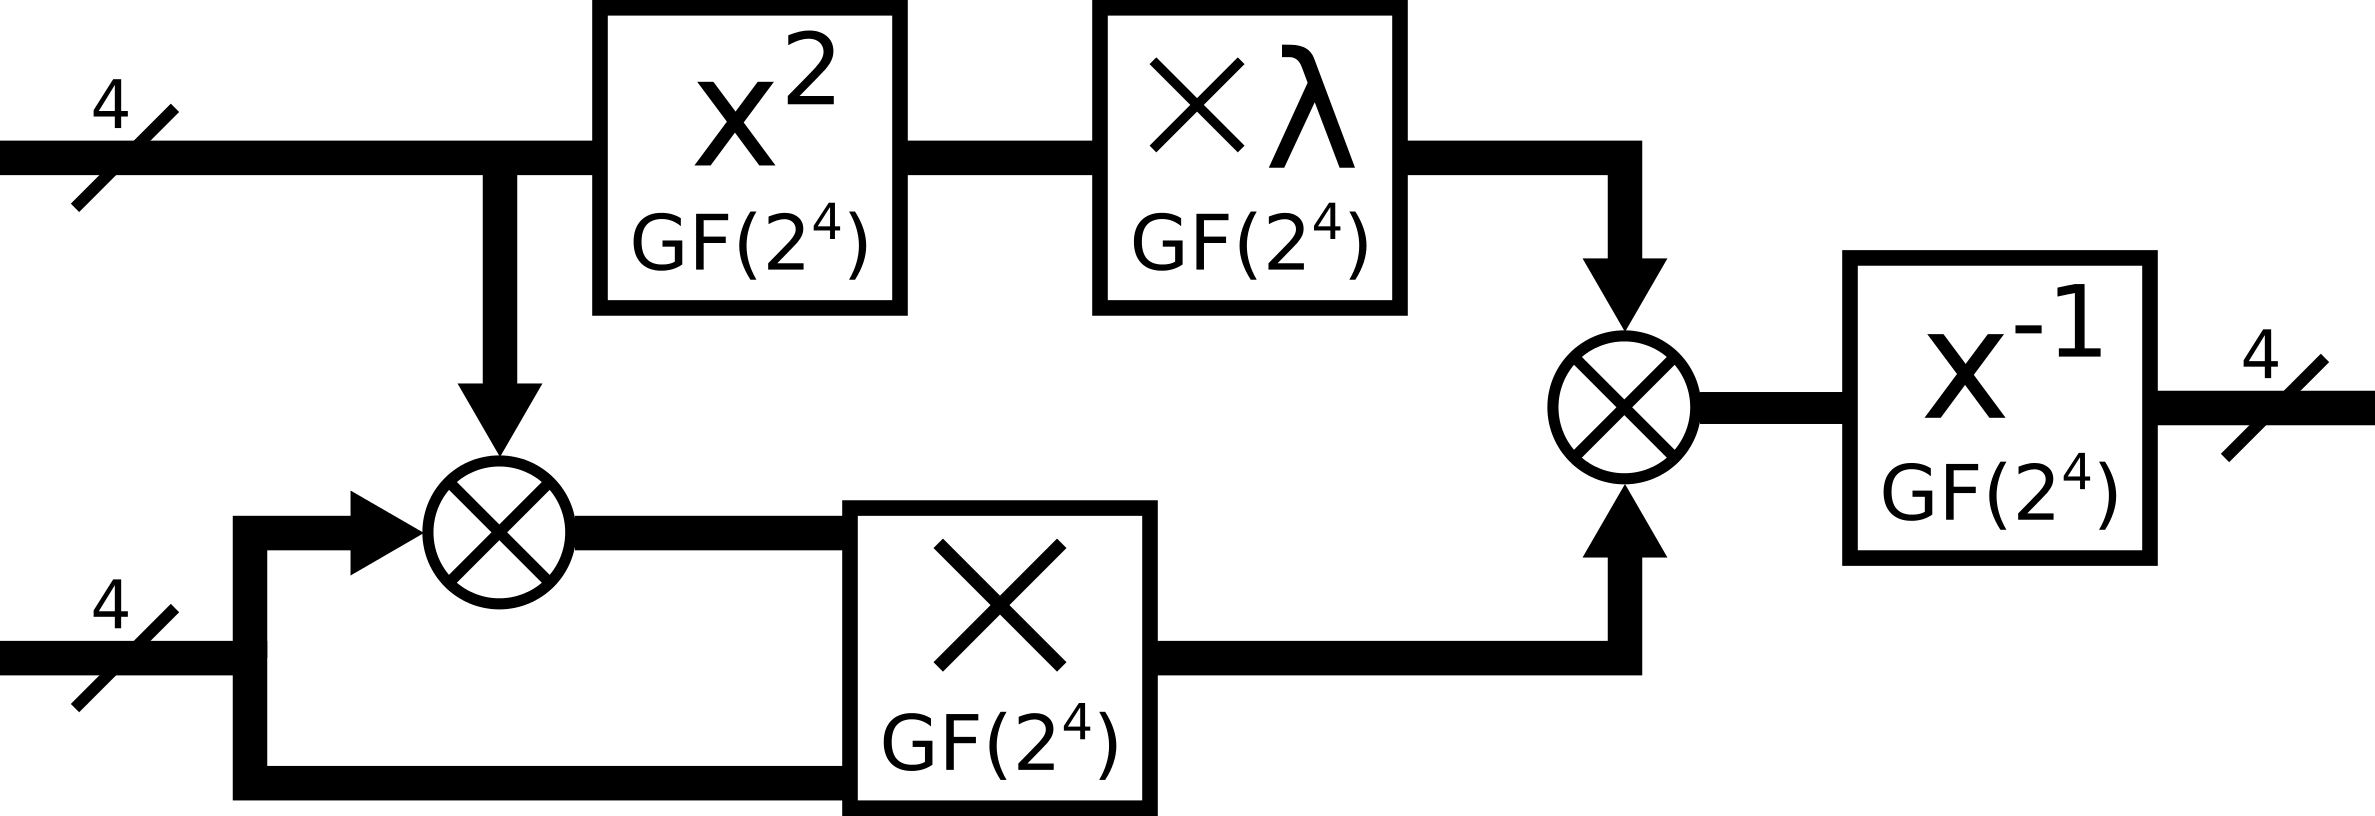
\includegraphics[scale=3]{theta-gf4}
\caption{Theta calculation circuit}
\end{figure}

\begin{figure}
\label{fig:mul_inv_gf242}
\centering
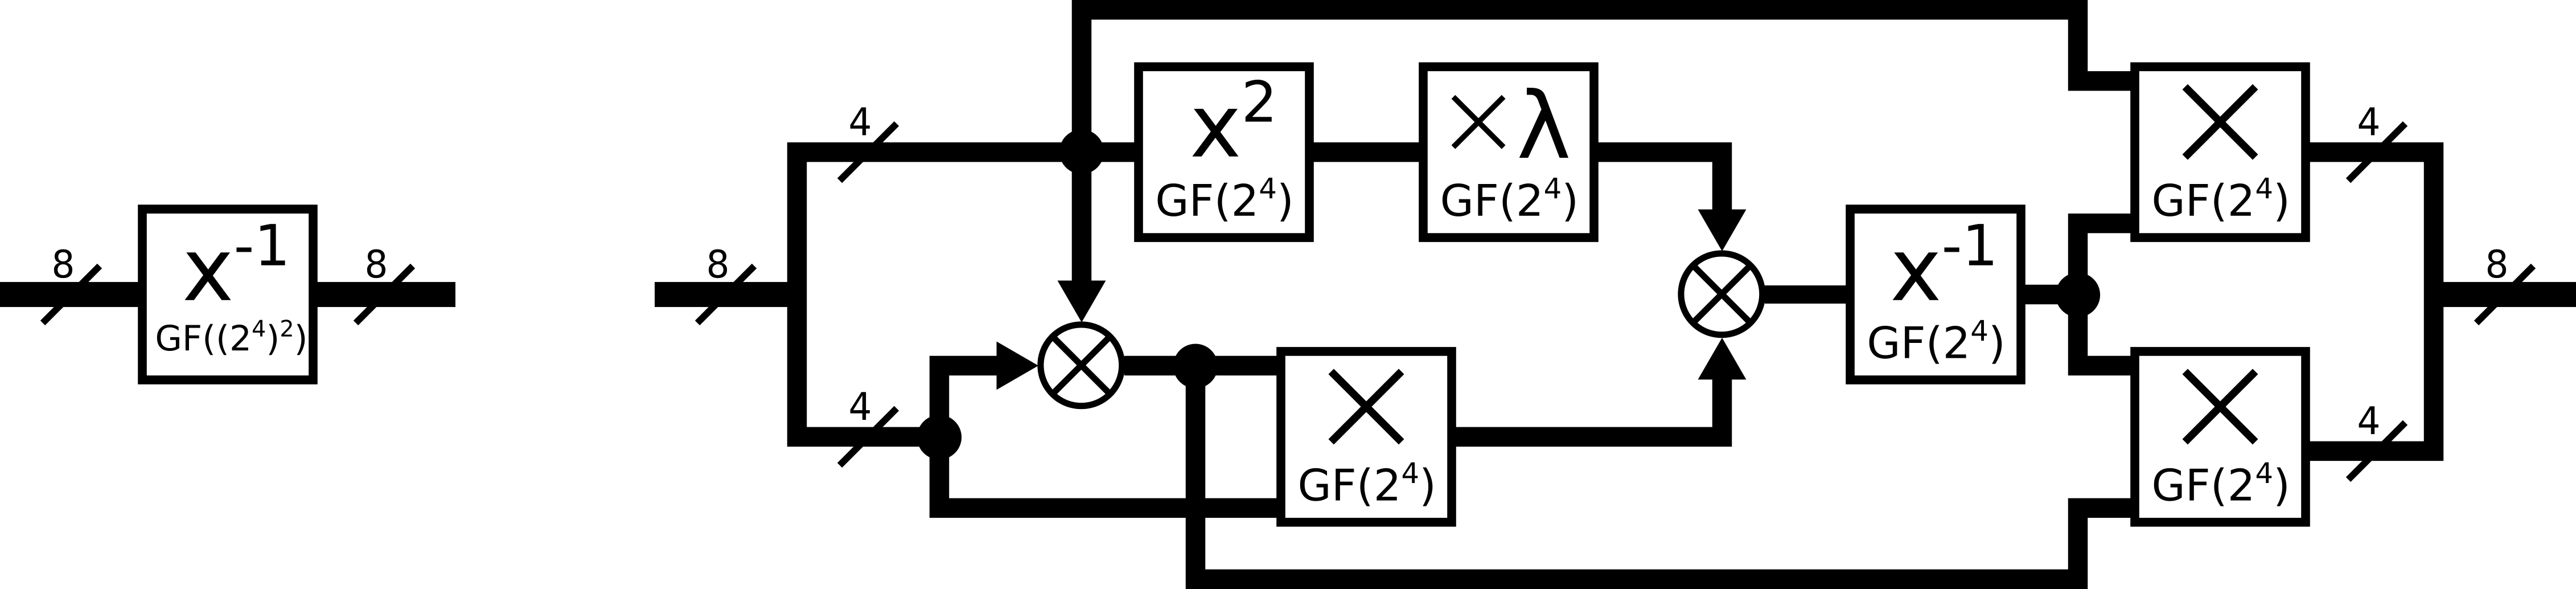
\includegraphics[scale=3]{inv-gf8}
\caption{Multiplicative inversion in $GF((2^4)^2)$ circuit}
\end{figure}

Operations to which multiplicative inversion in $GF((2^4)^2)$ is decomposed to are in $GF(2^4)$ and as a result the complecity of the solution is decreased. Some of those blocks are efficient to implement in hardware directly, and others can be decomposed even further.

\paragraph{Multiplicative inversion in $GF(2^4)$}\mbox{}\\
Authors of \cite{vlsi} derived that multiplicative inversion of $\{x_3x_2x_1x_0\} \in GF(2^4)$ can be calculated using formula (\ref{eq:mul_inf_gf24}).
\begin{equation}
\label{eq:mul_inf_gf24}
\begin{aligned}
x_3^{-1} &= x_3 + x_1x_2x_3 + x_0x_3 + x_2\\
x_2^{-1} &= x_1x_2x_3 + x_0x_2x_3 + x_0x_3 + x_2 + x_1x_2\\
x_1^{-1} &= x_3 + x_1x_2x_3 + x_0x_1x_3 + x_2 + x_0x_2 + x_1\\
x_0^{-1} &= x_1x_2x_3 + x_0x_2x_3 + x_1x_3 + x_0x_1x_3 + x_0x_3 + x_2 + x_1x_2 + x_0x_1x_2 + x_1 + x_0
\end{aligned}
\end{equation}

This can be further optimized for hardware implementation using substructure sharing (\ref{eq:mul_inf_gf24_opt}), which reduces the number of required operations to 9 multiplications ($and$ gates) and 14 additions ($xor$ gates).
\begin{equation}
\label{eq:mul_inf_gf24_opt}
\begin{aligned}
x_{01}   &= x_0x_1                             \\
x_{02}   &= x_0x_2                             \\
x_{03}   &= x_0x_3                             \\
x_{12}   &= x_1x_2                             \\
x_{13}   &= x_1x_3                             \\
x_{123}  &= x_{12}x_3                          \\
x_{023}  &= x_{02}x_3                          \\
x_{013}  &= x_{01}x_3                          \\
x_{012}  &= x_{01}x_2                          \\
a        &= x_{123} + x_2                      \\
b        &= a + x_{03}                         \\
c        &= x_{023} + x_{12}                   \\
d        &= x_{013} + x_{1}                    \\
x_3^{-1} &= b + x_3                            \\
x_2^{-1} &= b + c                              \\
x_1^{-1} &= a + d + x_3 + x_{02}               \\
x_0^{-1} &= b + c + d + x_{13} + x_{012} + x_0
\end{aligned}
\end{equation}


\begin{figure}
\label{fig:mul_inv_gf4_symbol}
\centering
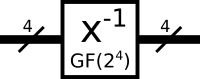
\includegraphics[scale=3]{inv-gf4-symbol}
\caption{Symbol of multiplicative inversion in $GF(2^4)$}
\end{figure}

In all diagrams symbol \ref{fig:mul_inv_gf4_symbol} will be used for multiplicative inversion in $GF(2^4)$


\paragraph{Multiplication by constant $\phi$ in $GF(2^2)$}\mbox{}\\
Lets first notice that for any $a \in GF(2^n)$ (\ref{eq:modulo_proof}) it is true. Keep in mind that coefficients of polynomials are in $GF(2^n)$ where addition is $xor$, so $(x + a) + (x + a) = 0$. This will be useful for decomposing operations between fields (\ref{eq:comp_fields_and_polys}) in deriving efficient circuits for them.
\begin{equation}
\label{eq:modulo_proof}
\begin{aligned}
x^2 &= (x^2 + x + a) + (x + a) &\\
x^2 &= (x + a)                 &\mod  x^2 + x + a
\end{aligned}
\end{equation}

As defined in (\ref{eq:comp_fields_and_polys}) \cite{vlsi} $\phi = \{10\}$. Product $k = \{k_1k_0\} \in GF(2^2)$ of $v = \{v_1v_0\} \in GF(2^2)$ by $\phi$ can be calculated as in \ref{eq:mul_phi}.

\begin{equation}
\label{eq:mul_phi}
\begin{aligned}
\phi v = x (v_1x + v_0) = v_1x^2 + v_0x &\stackrel{(\ref{eq:comp_fields_and_polys}, \ref{eq:modulo_proof})}{=} v_1(x + 1) + v_0x = (v_1 + v_0)x + v_1\\
k_1 &= v_1 + v_0\\
k_0 &= v_1
\end{aligned}
\end{equation}

It follows that multiplication by $\phi$ can be implemented as a circuit in fig. \ref{fig:phi_mul}.

\begin{figure}[!h]
\label{fig:phi_mul}
\centering
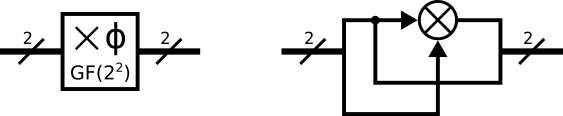
\includegraphics[scale=3]{mul-phi-gf2}
\caption{SubButes transformation decomposition}
\end{figure}


\paragraph{Multiplication by constant $\lambda$ in $GF(2^4)$}\mbox{}\\
As defined in (\ref{eq:comp_fields_and_polys}) \cite{vlsi} $\lambda = \{1100\} \in GF(2^4)$. Product $k = \{k_3k_2k_1k_0\} \in GF(2^4)$ of $v = \{v_3v_2v_1v_0\} \in GF(2^4)$ by $\lambda$ can be then calculated as in \ref{eq:mul_lambda}.

\begin{equation}
\label{eq:mul_lambda}
\begin{aligned}
\lambda v &= (\{11\}x) (\{v_3v_2\}x + \{v_1v_0\})\\
&= \{11\}\{v_3v_2\}x^2 + \{11\}\{v_1v_0\}x\\
&\stackrel{(\ref{eq:comp_fields_and_polys}, \ref{eq:modulo_proof})}{=}
\{11\}\{v_3v_2\}(x + \phi) + \{11\}\{v_1v_0\}x \\
&= (\{11\}\{v_3v_2\} + \{11\}\{v_1v_0\})x + \{11\}\{v_3v_2\}\phi\\
\{k_3k_2\} &= \{11\}\{v_3v_2\} + \{11\}\{v_1v_0\}\\
\{k_1k_0\} &= \{11\}\{v_3v_2\}\phi
\end{aligned}
\end{equation}

Multiplications of $\{v_1v_0\}$ and $\{v_3v_2\}$ by constant $\{11\}$ can be calculated similarly to multiplication by $\phi$ above (\ref{eq:mul_phi}).

\begin{equation}
\label{eq:mul_lambda_11}
\begin{aligned}
\{11\}\{v_bv_a\} &= (x + 1)(v_bx + v_a)\\
&= v_bx^2 + (v_b + v_a)x + v_a \\
&\stackrel{(\ref{eq:comp_fields_and_polys}, \ref{eq:modulo_proof})}{=}
v_b(x + 1) + (v_b + v_a)x + v_a \\
&= v_ax + (v_b + v_a)
\end{aligned}
\end{equation}

Combining (\ref{eq:mul_lambda}) and (\ref{eq:mul_lambda_11}) we can conclude (\ref{eq:mul_lambda2}).

\begin{equation}
\label{eq:mul_lambda2}
\begin{aligned}
\{k_3k_2\}
&\stackrel{(\ref{eq:mul_lambda_11})}{=}
(v_2x + (v_3 + v_2)) + (v_0x + (v_1 + v_0)) \\
&= (v_2 + v_0)x + (v_3 + v_2 + v_1 + v_0)\\
\{k_1k_0\}
&\stackrel{(\ref{eq:mul_lambda_11})}{=}
(v_2x + (v_3 + v_2))\phi \\
&\stackrel{(\ref{eq:mul_phi})}{=}
v_3x + v_2\\
k_3 &= v_2 + v_0\\
k_2 &= v_3 + v_2 + v_1 + v_0\\
k_1 &= v_3\\
k_0 &= v_2
\end{aligned}
\end{equation}


It follows that multiplication by $\lambda$ can be implemented as a circuit in fig. \ref{fig:lambda_mul}.

\begin{figure}[!h]
\label{fig:lambda_mul}
\centering
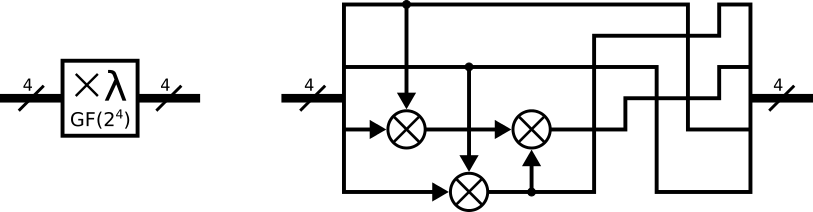
\includegraphics[scale=3]{mul-lam-gf4}
\caption{Constant multiplication by $\lambda$ circuit}
\end{figure}


\paragraph{Multiplication in $GF(2^2)$}\mbox{}\\
Product $k = \{k_1k_0\} \in GF(2^2)$ of $p = \{p_1p_0\} \in GF(2^2)$ by $q = \{q_1q_0\} \in GF(2^2)$ can be calculated as in (\ref{eq:mul_gf2}).

\begin{equation}
\label{eq:mul_gf2}
\begin{aligned}
pq &= (p_1x + p_0)(q_1x + q_0)\\
&= p_1q_1x^2 + (p_0q_1 + p_1q_0)x + p_0q_0\\
&\stackrel{(\ref{eq:comp_fields_and_polys}, \ref{eq:modulo_proof})}{=}
p_1q_1(x + 1) + (p_0q_1 + p_1q_0)x + p_0q_0\\
&=(p_1q_1 + p_0q_1 + p_1q_0)x + (p_1q_1 + p_0q_0)\\
k_1 &= p_1q_1 + p_0q_1 + p_1q_0\\
k_0 &= p_1q_1 + p_0q_0
\end{aligned}
\end{equation}

One can notice that for any $a, b, c, d \in GF(2^n)$ equation (\ref{eq:mul_gf_opt}) is always true.

\begin{equation}
\label{eq:mul_gf_opt}
\begin{aligned}
ad + bc + bd = (ac + ad + bc + bd) + ac = (a + b)(b + d) + ac
\end{aligned}
\end{equation}

To further reduce complexity of multiplication in $GF(2^2)$ by taking advantage of substructure sharing (of $p_0q_0$) and thus reducing overall number of used gates by 1, (\ref{eq:mul_gf_opt}) can be applied to (\ref{eq:mul_gf2}) ($a = p_0, b = p_1, c = q_0, d = q_1$).

\begin{equation}
\label{eq:mul_gf2_final}
\begin{aligned}
k_1 &= (p_0 + p_1)(q_0 + q_1) + p_0q_0\\
k_0 &= p_1q_1 + p_0q_0
\end{aligned}
\end{equation}


It follows that multiplication in $GF(2^2)$ (\ref{eq:mul_gf2_final}) can be implemented as a circuit in fig. \ref{fig:mul_gf2}.

\begin{figure}[!h]
\label{fig:mul_gf2}
\centering
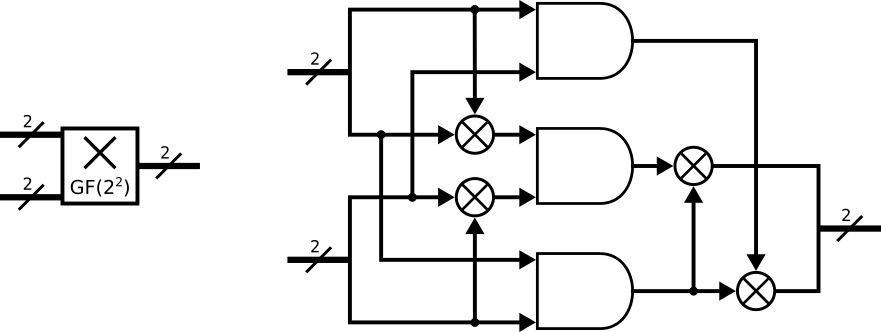
\includegraphics[scale=3]{mul-gf2}
\caption{Multiplication in $GF(2^2)$ circuit}
\end{figure}



\paragraph{Multiplication in $GF(2^4)$}\mbox{}\\
Product $k = \{k_3k_2k_1k_0\} \in GF(2^4)$ of $p = \{p_3p_2p_1p_0\} \in GF(2^4)$ by $q = \{q_3q_2q_1q_0\} \in GF(2^4)$ can be calculated as in (\ref{eq:mul_gf4}).

\begin{equation}
\label{eq:mul_gf4}
\begin{aligned}
pq &= (\{p_3p_2\}x + \{p_1p_0\})(\{q_3q_2\}x + \{q_1q_0\})\\
&= \{p_3p_2\}\{q_3q_2\}x^2 + (\{p_1p_0\}\{q_3q_2\} + \{p_3p_2\}\{q_1q_0\})x + \{p_1p_0\}\{q_1q_0\} \\
&\stackrel{(\ref{eq:comp_fields_and_polys}, \ref{eq:modulo_proof})}{=}
\{p_3p_2\}\{q_3q_2\}(x + \phi) + (\{p_1p_0\}\{q_3q_2\} + \{p_3p_2\}\{q_1q_0\})x + \{p_1p_0\}\{q_1q_0\} \\
&= (\{p_3p_2\}\{q_3q_2\} + \{p_1p_0\}\{q_3q_2\} + \{p_3p_2\}\{q_1q_0\})x + (\{p_3p_2\}\{q_3q_2\}\phi + \{p_1p_0\}\{q_1q_0\})\\
\{k_3k_2\} &= \{p_3p_2\}\{q_3q_2\} + \{p_1p_0\}\{q_3q_2\} + \{p_3p_2\}\{q_1q_0\}\\
\{k_1k_0\} &= \{p_3p_2\}\{q_3q_2\}\phi + \{p_1p_0\}\{q_1q_0\}
\end{aligned}
\end{equation}

To further reduce complexity of multiplication in $GF(2^4)$ by reducing number of $GF(2^2)$ multiplications (\ref{eq:mul_gf_opt}) can be applied to (\ref{eq:mul_gf4}) ($a = \{p_1p_0\}, b = \{p_3p_2\}, c = \{q_1q_0\}, d = \{q_3q_2\}$).

\begin{equation}
\label{eq:mul_gf4_final}
\begin{aligned}
\{k_3k_2\} &= (\{p_1p_0\} + \{p_3p_2\})(\{q_1q_0\} + \{q_3q_2\}) + \{p_1p_0\}\{q_1q_0\}\\
\{k_1k_0\} &= \{p_3p_2\}\{q_3q_2\}\phi + \{p_1p_0\}\{q_1q_0\}
\end{aligned}
\end{equation}



It follows that multiplication in $GF(2^4)$ can be implemented as a circuit in fig. \ref{fig:mul_gf4}.

\begin{figure}[!h]
\label{fig:mul_gf4}
\centering
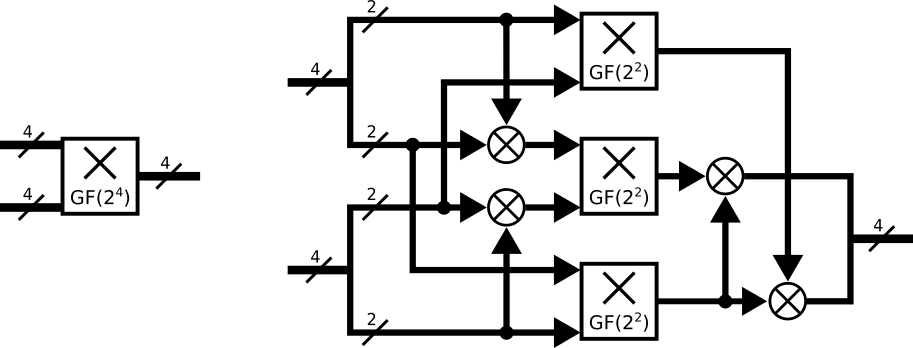
\includegraphics[scale=3]{mul-gf4}
\caption{Multiplication in $GF(2^4)$ circuit}
\end{figure}


\paragraph{Squaring in $GF(2^4)$}\mbox{}\\
Lets first establish how squaring in $GF(2^2)$ can be calculated. 
Square $s = \{s_1s_0\} \in GF(2^2)$ of $d = \{d_1d_0\} \in GF(2^2)$ can be calculated as in \ref{eq:gq_gf2}. Keep in mind that squating in $GF(2)$ is an $and$ operation and thus for any $l \in GF(2)$ it is true that $l^2 = l$.

\begin{equation}
\label{eq:sq_gf2}
\begin{aligned}
s^2 &= (d_1x + d_0)(d_1x + d_0) \\
&= d_1^2x^2 + (d_1d_0 + d_1d_0)x + d_0^2 \\
&= d_1^2x^2 + d_0^2 \\
&= d_1x^2 + d_0\\
&\stackrel{(\ref{eq:comp_fields_and_polys}, \ref{eq:modulo_proof})}{=}
d_1(x + 1) + d_0 \\
&= d_1x + (d_1 + d_0)\\
s_1 &= d_1\\
s_0 &= d_1 + d_0
\end{aligned}
\end{equation}

Square $k = \{k_3k_2k_1k_0\} \in GF(2^4)$ of $v = \{v_3v_2v_1v_0\} \in GF(2^4)$ can be calculated as in \ref{eq:sq_gf4}.

\begin{equation}
\label{eq:sq_gf4}
\begin{aligned}
k^2 &= (\{v_3v_2\}x + \{v_1v_0\})(\{v_3v_2\}x + \{v_1v_0\})\\
&= \{v_3v_2\}^2x^2 + (\{v_3v_2\}\{v_1v_0\} + \{v_3v_2\}\{v_1v_0\})x + \{v_1v_0\}^2 \\
&= \{v_3v_2\}^2x^2 + \{v_1v_0\}^2 \\
&\stackrel{(\ref{eq:comp_fields_and_polys}, \ref{eq:modulo_proof})}{=}
\{v_3v_2\}^2(x + \phi) + \{v_1v_0\}^2 \\
&= \{v_3v_2\}^2x + (\{v_1v_0\}^2 + \{v_3v_2\}^2\phi)\\
\{k_3k_2\} &= \{v_3v_2\}^2 \\
\{k_1k_0\} &= \{v_1v_0\}^2 + \{v_3v_2\}^2\phi
\end{aligned}
\end{equation}

Applying (\ref{eq:sq_gf2}) to (\ref{eq:sq_gf4}) yields final formula (\ref{eq:sq_gf4_final}), which can be implemented in hardware as a circuit \ref{fig:sq_sq4}.
\begin{equation}
\label{eq:sq_gf4_final}
\begin{aligned}
\{k_3k_2\} &= \{v_3v_2\}^2 = (v_3x + v_2)^2
\stackrel{(\ref{eq:sq_gf2})}{=}
v_3x + (v_3 + v_2)\\
\{k_1k_0\} &= \{v_1v_0\}^2 + \{v_3v_2\}^2\phi \\
&= (v_1x + v_0)^2 + (v_3x + v_2)^2\phi \\
&\stackrel{(\ref{eq:sq_gf2})}{=}
(v_1x + (v_1 + v_0)) + (v_3x + (v_3 + v_2))\phi \\
&\stackrel{(\ref{eq:mul_phi})}{=}
(v_1x + (v_1 + v_0)) + (v_2x + v_3)) \\
&= (v_2 + v_1)x + (v_3 + v_1 + v_0) \\
k_3 &= v_3 \\
k_2 &= v_3 + v_2 \\
k_1 &= v_2 + v_1 \\
k_0 &= v_3 + v_1 + v_0
\end{aligned}
\end{equation}

\begin{figure}[!h]
\label{fig:mul_sq4}
\centering
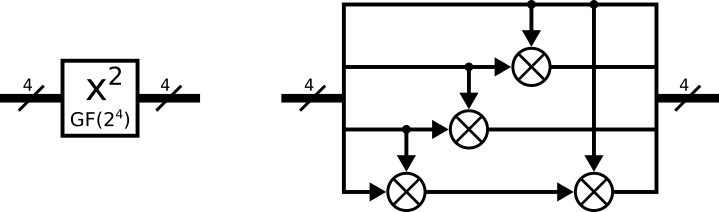
\includegraphics[scale=3]{sq-gf4}
\caption{Squaring in $GF(2^4)$ circuit}
\end{figure}
